Tcpdump --- это консольная утилита Unux для перехвата и анализа сетевого трафика. Необходимо при запуске программы указать ей сетевой интерфейс, который будет прослушиваться. В нашем случае это Wi-Fi-адаптер (wlan0).

Напишем bash-скрипт со следующей командой:

\begin{verbatim}
$ #!/bin/bash
$ sudo tcpdump -v -i wlan0 -s 0 -w /tmp/sniff.pcap -c <число_пакетов>
\end{verbatim}

Параметр -c задает максимальное количество пакетов для перехвата, после чего система останавливает выполнение скрипта.

Результат выполнения tcpdump записывается в файл /tmp/sniff.pcap. Pcap --- это универсальный формат, который позволит в дальнейшем проанализировать перехваченный трафик в других программах.

После этого необходимо скопировать полученный pcap-файл на основную машину с Ubuntu для дальнейшего анализа в программе Wireshark. Сделать это можно при момощи команды scp (рис.~\ref{tcpdump_1:tcpdump_1}).

\begin{figure}[h!]
\center{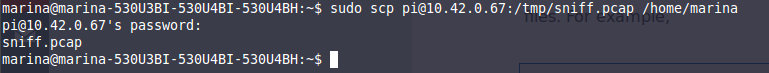
\includegraphics[width=0.6\linewidth]{tcpdump_1}}
\caption{ Копирование pcap-файла по ssh-соединению }
\label{tcpdump_1:tcpdump_1}
\end{figure}

\clearpage



